\PassOptionsToPackage{dvipsnames}{xcolor}
\documentclass{beamer}
\beamertemplatenavigationsymbolsempty
\usecolortheme{beaver}
\setbeamertemplate{blocks}[rounded=true, shadow=true]
\setbeamertemplate{footline}[page number]
% \usepackage[dvipsnames]{xcolor}

\usepackage[utf8]{inputenc}
\usepackage[english,russian]{babel}
\usepackage{amssymb,amsfonts,amsmath,mathtext}
\usepackage{algorithm}
\usepackage{algpseudocode}
\makeatletter
\renewcommand{\ALG@name}{Алгоритм}
\makeatother

\DeclareMathOperator*{\argmin}{arg\,min}
\DeclareMathOperator*{\argmax}{arg\,max}

%----------------------------------------------------------------------------------------------------------

\title[\hbox to 56mm{Аппроксимации градиента с помощью оракула нулевого порядка и техники запоминания}]{Аппроксимации градиента с помощью оракула нулевого порядка и техники запоминания}
\author[Богданов А. И.]{Богданов Александр Иванович \\
                        $ $ \\
                        Научный руководитель: \\
                        к.ф.-м.н. Безносиков А. Н.}
\institute[]{Кафедра <<Интеллектуальные системы>> \\ 
             $ $ \\
             03.03.01~--- Прикладные математика и физика \\
             $ $ \\
             Московский физико-технический институт \\
             (национальный исследовательский университет) \\
             Физтех-школа прикладной математики и информатики \\}
\date{}

%----------------------------------------------------------------------------------------------------------

\begin{document}

%----------------------------------------------------------------------------------------------------------

\begin{frame}

    \maketitle

\end{frame}

%-----------------------------------------------------------------------------------------------------

\begin{frame}{Цель исследования}

    \textbf{Проблема:} Ставится задача оптимизации с доступом только к зашумленному нулевому оракулу. \\

    $ $\\

    \textbf{Цель:} Предложить робастый алгоритм аппроксимации градиента, использующий $\mathcal{O}(1)$ вызовов оракула на каждой итерации.\\

    $ $\\

    \textbf{Решение:} Предлагается аппроксимация градиента \texttt{JAGUAR}, которая использует технику запоминания.
    
\end{frame}

%-----------------------------------------------------------------------------------------------------

\begin{frame}{Постановка задачи}

    Рассматривается две оптимизационные задачи:

    \begin{itemize}
        \item Нестохастическая
                
            \begin{align*}
                \min_{x \in Q} f(x)
            \end{align*}

            Доступ только к $f_{\delta}(x) := f(x) + \delta(x)$, где $\delta(x)$ -- шум.

        \item Стохастическая
        
            \begin{align*}
                \min_{x \in Q} f(x) :=  \mathbb{E}_{\xi \sim \pi} \left[ f(x, \xi) \right]
            \end{align*}

                
            Доступ только к $f_{\delta}(x, \xi) := f(x, \xi) + \delta(x, \xi)$, где $\delta(x, \xi)$ - шум.

    \end{itemize}

    Множество $Q \subseteq \mathbb{R}^d$ -- произвольное.
   
\end{frame}

%-----------------------------------------------------------------------------------------------------

\begin{frame}{\texttt{JAGUAR-d}}

    Схема аппроксимации:
    \begin{align*}
        \widetilde{\nabla}_i f_\delta (x) :=  \frac{f_\delta (x + \tau e_i) - f_\delta(x - \tau e_i)}{2 \tau} e_i,
    \end{align*}
    где $e_i$ -- $i$-ый базисный вектор, $\tau$ -- параметр сглаживания.
    
    \begin{algorithm}[H]
        \caption{}
        \begin{algorithmic}[1]
            \State \textbf{Вход:} $x, h \in \mathbb{R}^d$
            \State Сэмплируем $i \in \overline{1, d}$ равномерно и независимо
            \State Считаем $\widetilde{\nabla}_i f_\delta (x) = \frac{f_\delta (x + \tau e_i) - f_\delta (x - \tau e_i)}{2 \tau} e_i$
            \State $h = h - \langle h, e_i \rangle e_i + \widetilde{\nabla}_i f_\delta (x)$
            \State \textbf{Выход:} $h$
        \end{algorithmic}
    \end{algorithm}
        
\end{frame}

%----------------------------------------------------------------------------------------------------------

\begin{frame}{\texttt{JAGUAR-s}}
    Схемы аппроксимации:
        \begin{align*}
            \widetilde{\nabla}_i f_\delta (x, \xi^+, \xi^-) :=  \frac{f_\delta (x + \tau e_i, \xi^+) - f_\delta (x - \tau e_i, \xi^-)}{2 \tau} e_i,
        \end{align*}
    где $e_i$ -- $i$-ый базисный вектор, $\tau$ -- параметр сглаживания.
    
    При $\xi^+ \not = \xi^-$ -- одноточечная обратная связь (ООС), а при $\xi^+ = \xi^-$ -- двухточечная обратная связь (ДОС).
    
    \begin{algorithm}[H]
        \caption{}
        \begin{algorithmic}[1]
            \State \textbf{Вход:} $x, h, g \in \mathbb{R}^d$; $\eta \in [0, 1]$
            \State Сэмплируем $i \in \overline{1, d}$ равномерно и независимо
            \State Сэмплируем $\xi$: $\xi^+$ и $\xi^-$ независимо (в ДОС $\xi^+ = \xi^-$)
            \State Считаем $\widetilde{\nabla}_i f_\delta (x, \xi^\pm) = \frac{f_\delta (x + \tau e_i, \xi^+) - f_\delta (x - \tau e_i, \xi^-)}{2 \tau} e_i$
            \State $h = h - \langle h, e_i \rangle e_i + \widetilde{\nabla}_i f_\delta (x, \xi^+, \xi^-)$
            \State $\rho = h - d \cdot \langle h, e_i \rangle e_i + d \cdot \widetilde{\nabla}_i f_\delta (x, \xi^+, \xi^-)$
            \State $g = (1 - \eta) g + \eta \rho$ 
            \State \textbf{Выход:} $g, h$
        \end{algorithmic}
    \end{algorithm}
\end{frame}

%----------------------------------------------------------------------------------------------------------

\begin{frame}{Обычный алгоритм Франка-Вульфа}

    Общие допущения:
    \begin{enumerate}
        \item Ограниченность множества $Q$:
            \begin{align*}
                \forall x, y \in Q: \|x - y\|^2 \leq D^2.
            \end{align*}
        \item Выпуклость множества $Q$:
            \begin{align*}
                \forall 0 \leq \alpha \leq 1, \forall x, y \in Q: \alpha x + (1 - \alpha) y \in Q.
            \end{align*}
    \end{enumerate}

    \begin{algorithm}[H]
        \caption{}
        \begin{algorithmic}[1]
            \State {\bf Вход:} $x_0 \in Q$, $\gamma_k$
        	\For {k = 0, 1, 2, ... , N}
                \State $s^k = \argmin\limits_{s \in Q}  \left<s, \nabla f(x^k) \right>$
                \State $x^{k+1} = x^k + \gamma_k (s^k - x^k)$
            \EndFor
            \State {\bf Выход:} $x^{N + 1}$ 
        \end{algorithmic}
    \end{algorithm}

\end{frame}

%----------------------------------------------------------------------------------------------------------

\begin{frame}{Алгоритм Франка-Вульфа с \texttt{JAGUAR-d}}

    Допущения:
    \begin{enumerate}
        \item Функция $f(x)$ $L$-гладкая на множестве $Q$: 
            \begin{align*}
                \forall x, y \in Q: \left\| \nabla f(x) - \nabla f(y) \right\| \leq L \left\| x - y \right\|.
            \end{align*}

        \item Функция $f(x)$ выпукла на множестве $Q$:
            \begin{align*}
                \forall x, y \in Q: f(y) \geq f(x) + \langle \nabla f(x), y - x \rangle.
            \end{align*}

        \item Ограниченность оракульного шума:
            \begin{align*}
                \exists \Delta > 0 \forall x \in Q: | \delta(x) |^2 \leq \Delta^2.
            \end{align*}
                
    \end{enumerate}

\end{frame}

%----------------------------------------------------------------------------------------------------------

\begin{frame}{Алгоритм Франка-Вульфа с \texttt{JAGUAR-d}}

    \begin{algorithm}[H]
        \caption{}
        \begin{algorithmic}[1]
        	\State \textbf{Вход:} $x^0 \in Q$, $h^0 = \widetilde{\nabla} f_\delta (x^0)$, $\gamma_k$, $\tau$
        	\For {$k = 0, 1, 2, ... , N$}
                \State $h^{k + 1}$ = \texttt{JAGUAR-d} $\left( x^k, h^k \right)$
                \State $s^k = \argmin\limits_{x \in Q} \left< s, h^{k + 1} \right>$
                \State $x^{k + 1} = x^k + \gamma_k (s^k - x^k)$
            \EndFor
            \State \textbf{Вход:} $x^{N + 1}$
        \end{algorithmic}
    \end{algorithm}

\end{frame}

%----------------------------------------------------------------------------------------------------------

\begin{frame}{Алгоритм Франка-Вульфа с \texttt{JAGUAR-d}}

    \textbf{Теорема (Богданов А., 2023)} При шаге оптимизатора:
    \begin{align*}
        \gamma_k = \frac{4}{k + 8d},
    \end{align*}  
    получается оценка на сходимость:
    \small{
        \begin{align*}
            \mathbb{E} \left[ f(x^{N}) - f(x^*) \right] = \mathcal{O} \left( \frac{d \max\{L D^2, f(x^0) - f(x^*)\}}{N + 8d} + \sqrt{d} L D \tau + \frac{\sqrt{d} \Delta D}{\tau}\right).
            \end{align*}
    }
    
    \textbf{Следствие} Пусть $\varepsilon$ определяет точность: $\mathbb{E} \left[f(x^N) - f(x^*) \right] \leq \varepsilon$:
    \begin{align*}
        N = \mathcal{O} \left( \frac{d \max\{L D^2, f(x^0) - f(x^*)\}}{\varepsilon} \right),
    \end{align*}
    \begin{align*}
        \gamma = \mathcal{O} \left(\frac{\varepsilon}{\sqrt{d} L D} \right), \quad
        \Delta = \mathcal{O} \left( \frac{\varepsilon^2}{d L D^2}\right).
    \end{align*}

\end{frame}

%----------------------------------------------------------------------------------------------------------

\begin{frame}{Алгоритм Франка-Вульфа с \texttt{JAGUAR-s}}

    Допущения:
    \small{
        \begin{enumerate}
            \item Функция $f(x, \xi)$ $L(\xi)$-гладкая на множестве $Q$: 
                \begin{align*}
                    \forall\ x, y \in Q: \left\| \nabla f(x, \xi) - \nabla f(y, \xi) \right\| \leq L(\xi) \left\|x-y\right\|.
                \end{align*}
            \item Функция $f(x, \xi)$ выпукла на множестве $Q$:
                \begin{align*}
                    \forall\ x, y \in Q: f(y, \xi) \geq f(x, \xi) + \langle \nabla f(x, \xi), y - x \rangle.
                \end{align*}
            \item Ограниченность оракульного шума:
                \begin{align*}
                    \exists\ \Delta > 0: \forall\ x \in Q: \mathbb{E} \left[ |\delta(x, \xi)|^2 \right] \leq \Delta^2
                \end{align*}
            \item Ограниченность второго момента градиента:
                \begin{align*}
                    \exists\ \sigma^2_{\nabla}: \mathbb{E} \left[ \| \nabla f(x, \xi) - \nabla f(x) \|^2 \right] \leq \sigma^2_{\nabla}
                \end{align*}
            \item Ограниченность второго момента оракула (для ООС):
                \begin{align*}
                    \exists\ \sigma^2_{f}: \mathbb{E} \left[ \left|f(x, \xi) - f(x) \right|^2 \right] \leq \sigma^2_{f}
                \end{align*}
        \end{enumerate}
    }

\end{frame}

%----------------------------------------------------------------------------------------------------------

\begin{frame}{Алгоритм Франка-Вульфа с \texttt{JAGUAR-s}}

    \begin{algorithm}[H]
        \caption{Стохастический алгоритм Франка-Вульфа с \texttt{JAGUAR}} \label{alg:FW_stoch}
        \begin{algorithmic}[1]
        	\State \textbf{Вход:} $x^0 \in Q$, $h^0 = g^0 = \widetilde{\nabla} f_\delta (x^0)$, $\gamma_k$, $\eta_k$, $\tau$
        	\For {$k = 0, 1, 2, ... , N$}
                \State $g^{k + 1}$, $h^{k + 1}$ = \texttt{JAGUAR-s} $\left( x^k, h^k, g^k, \eta_k \right)$
                \State $s^k = \argmin\limits_{x \in Q} \left< s, g^{k + 1} \right>$
                \State $x^{k + 1} = x^k + \gamma_k (s^k - x^k)$
            \EndFor
            \State \textbf{Вход:} $x^{N + 1}$
        \end{algorithmic}
    \end{algorithm}
  
\end{frame}

%----------------------------------------------------------------------------------------------------------

\begin{frame}{Алгоритм Франка-Вульфа с \texttt{JAGUAR-s}}

    \textbf{Теорема (Богданов А., 2023)} При шаге оптимизатора и шаге моментума:
    \begin{align*}
        \gamma_k = \frac{4}{k + 8d^{3/2}}, \quad \eta_k = \frac{4}{(k + 8d^{3/2})^{2/3}}
    \end{align*}
    получается оценка на сходимость:
    \small{
        \begin{align*}
            \mathbb{E}\left[f(x^{N}) - f(x^*) \right] = \mathcal{O}
            &\Bigg(
            \frac{L D^2 + d \sigma_f D/ \tau + d \sigma_{\nabla} D + \sqrt{d} (f(x^0) - f(x^*))}{(N + 8d^{3/2})^{1/3}} \\
            &+
            \sqrt{d} L D \tau + \frac{\sqrt{d} \Delta D}{\tau} \Bigg)
        \end{align*}
    }
    \textbf{Следствие} Пусть $\varepsilon$ определяет точность: $\mathbb{E} \left[ f(x^N) - f(x^*) \right] \leq \varepsilon$:
    \begin{align*}
        N = \mathcal{O} \left( \max\left\{ \left[ \frac{L D^2 + d\sigma_{\nabla} D + \sqrt{d} (f(x^0) - f(x^*))}{\varepsilon}\right]^3 , \frac{d^{9/2} \sigma_f^3 L^3D^6}{\varepsilon^6} \right\}\right),
    \end{align*}
    \begin{align*}
        \gamma = \mathcal{O} \left(\frac{\varepsilon}{\sqrt{d} L D} \right), \quad \Delta = \mathcal{O} \left( \frac{\varepsilon^2}{d L D^2}\right).
    \end{align*}
            
\end{frame}

%----------------------------------------------------------------------------------------------------------

\begin{frame}{Постановка эксперимента}

    На множестве $Q$ рассматриваются модели LogReg и SVM вида:
    \begin{align*}
        \min_{w \in Q} \left\{ f(w) = \frac{1}{m} \sum_{k = 1}^{m} \log \left( 1 + \exp \left[ -y_k (Xw)_k \right] \right) + \frac{1}{2C} \| w \|^2 \right\}; \\
        \min_{w \in Q, b \in \mathbb{R}} \left\{ f(w, b) = \frac{1}{m} \sum_{k = 1}^{m} \left( 1 - y_k [(Xw)_k - b] \right)_+ + \frac{1}{2C} \| w \|^2 \right\}.
    \end{align*}

    Эксперимент проводится с регуляризационным членом $C = 10$, на множествах: симплексе $\Delta_d$ и $l_2$-шаре; датасете MNIST.
    
    В качестве базовых оценок градиента рассматриваются $l_2$-\textit{сглаживание} и \textit{полная аппроксимация}.

    Рассматривался шум:
    \begin{itemize}
        \item Стохастический: $f_\delta(x) = \text{round}(f(x), 5)$;
        \item Детерминированный: $f_\delta(x, \xi) = f(x) + \xi; \xi \sim \mathcal{N}(0, 0.1)$.
    \end{itemize}

\end{frame}

%----------------------------------------------------------------------------------------------------------

\begin{frame}{Эксперимент для нестохастического случая}

    \begin{figure}[H]
        \centering
        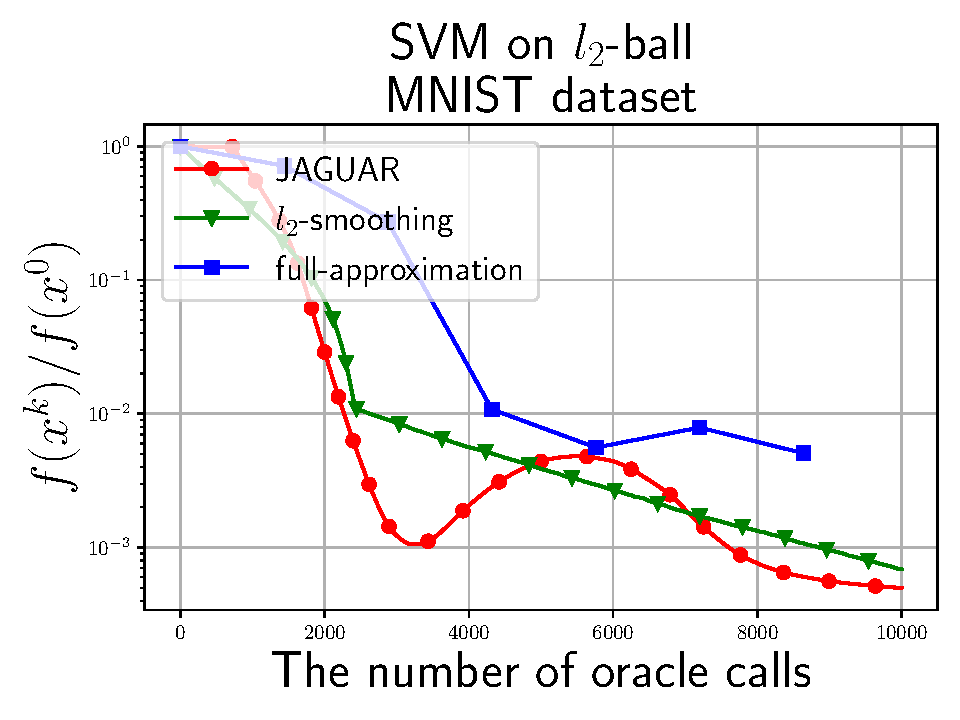
\includegraphics[width=0.49\textwidth]{figures/None_stochastics_FW_SVM_L2_MNIST.pdf}
        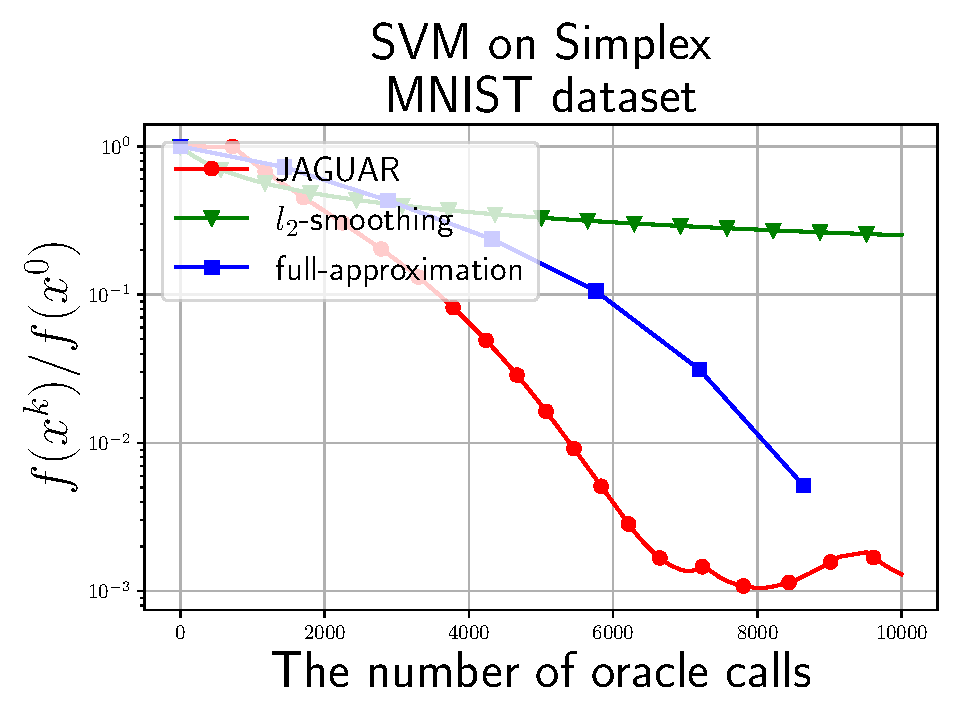
\includegraphics[width=0.49\textwidth]{figures/None_stochastics_FW_SVM_Simplex_MNIST.pdf}

        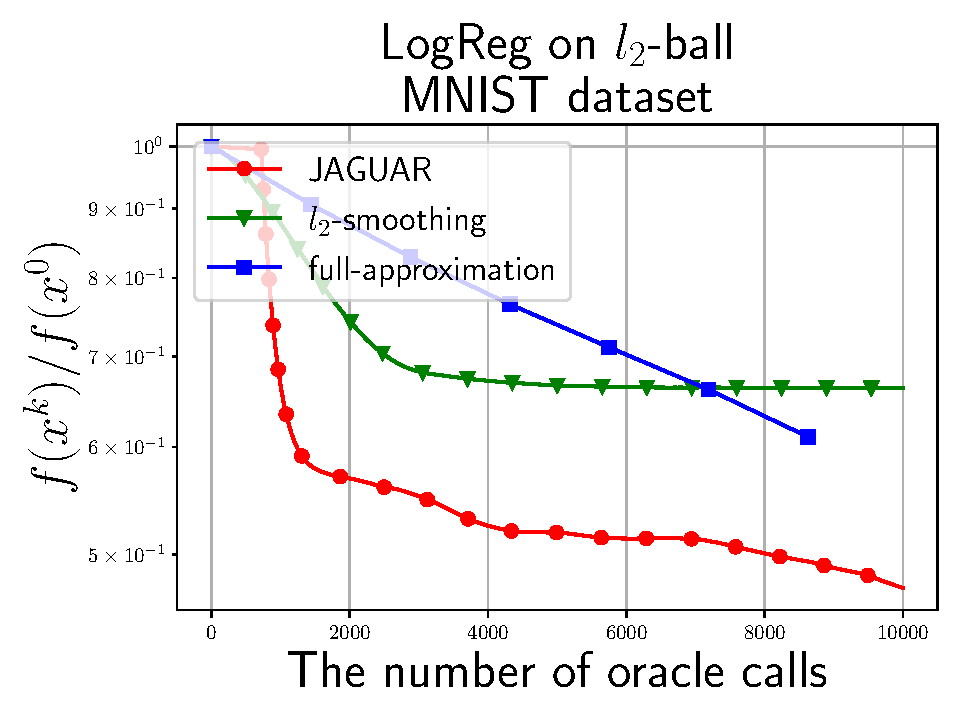
\includegraphics[width=0.49\textwidth]{figures/None_stochastics_FW_LogReg_L2_MNIST.pdf}
        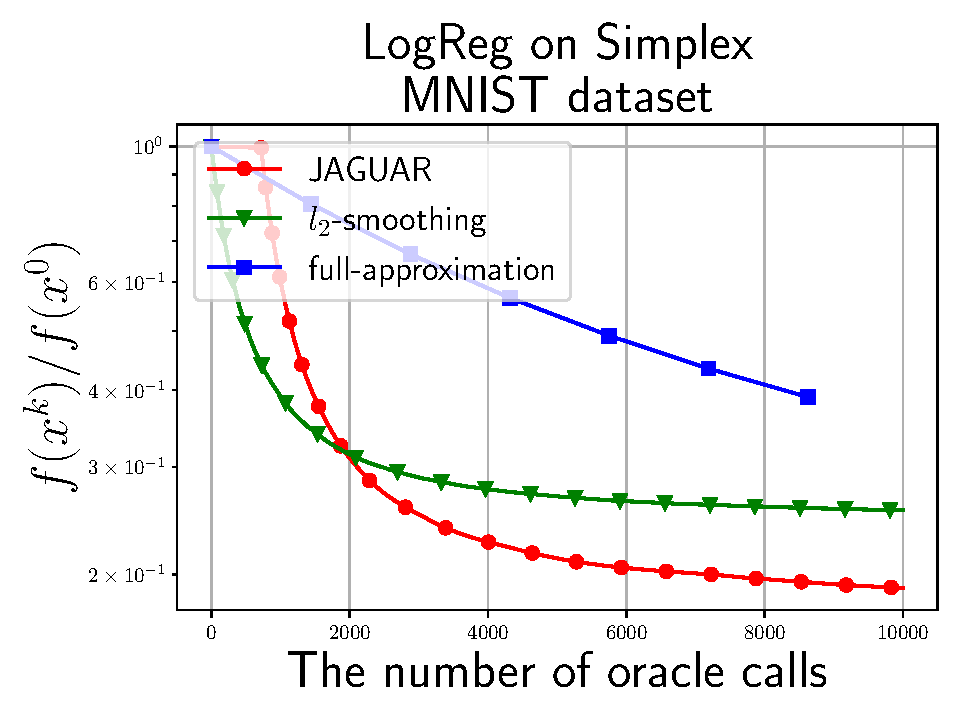
\includegraphics[width=0.49\textwidth]{figures/None_stochastics_FW_LogReg_Simplex_MNIST.pdf}
        
    \end{figure}

\end{frame}

%----------------------------------------------------------------------------------------------------------

\begin{frame}{Эксперимент для стохастического случая}

    \begin{figure}[H]
        \centering
        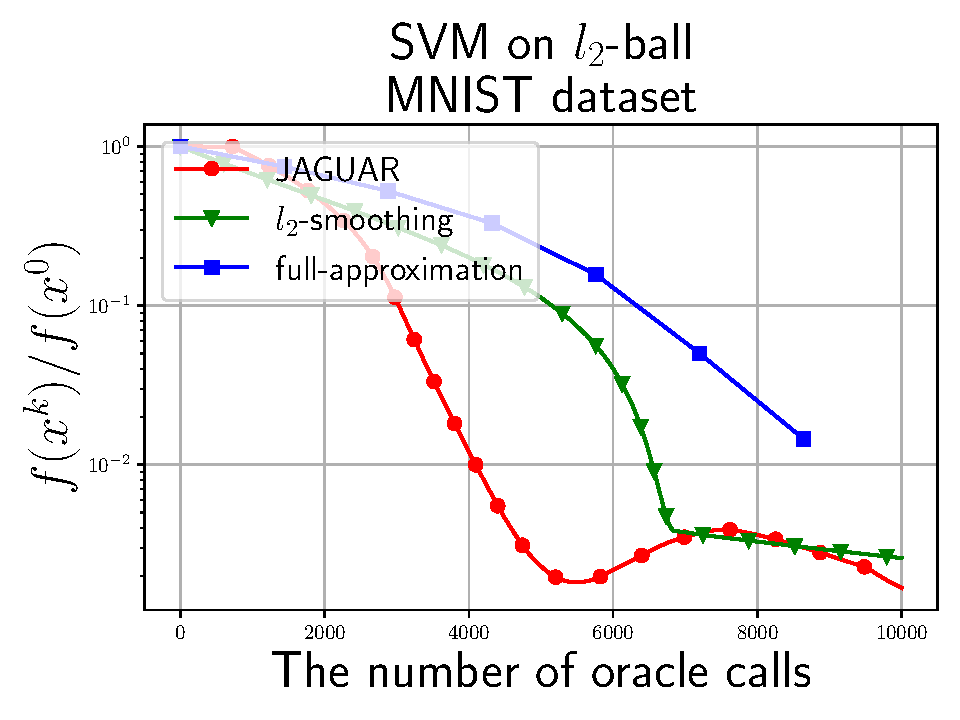
\includegraphics[width=0.49\textwidth]{figures/Stochastics_TPF_FW_SVM_L2_MNIST.pdf}
        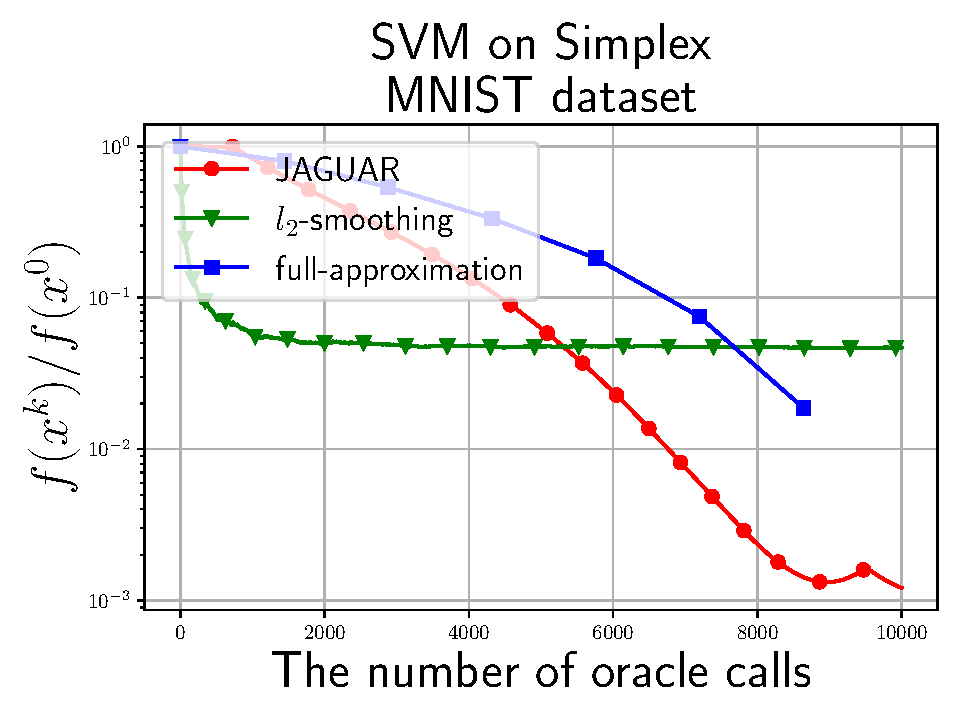
\includegraphics[width=0.49\textwidth]{figures/Stochastics_TPF_FW_SVM_Simplex_MNIST.pdf}

        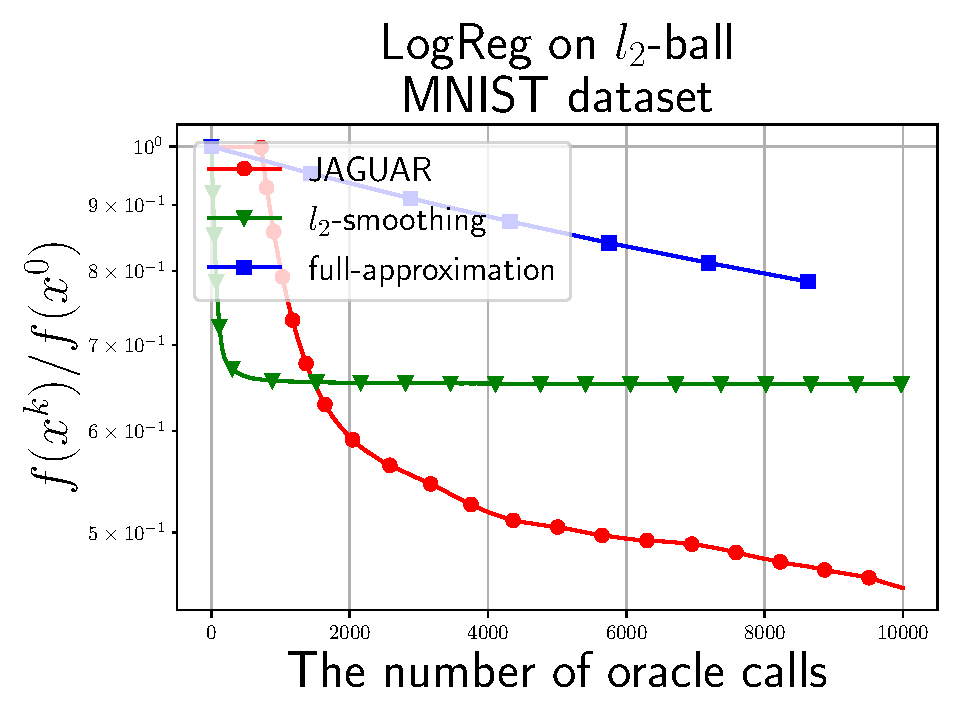
\includegraphics[width=0.49\textwidth]{figures/Stochastics_TPF_FW_LogReg_L2_MNIST.pdf}
        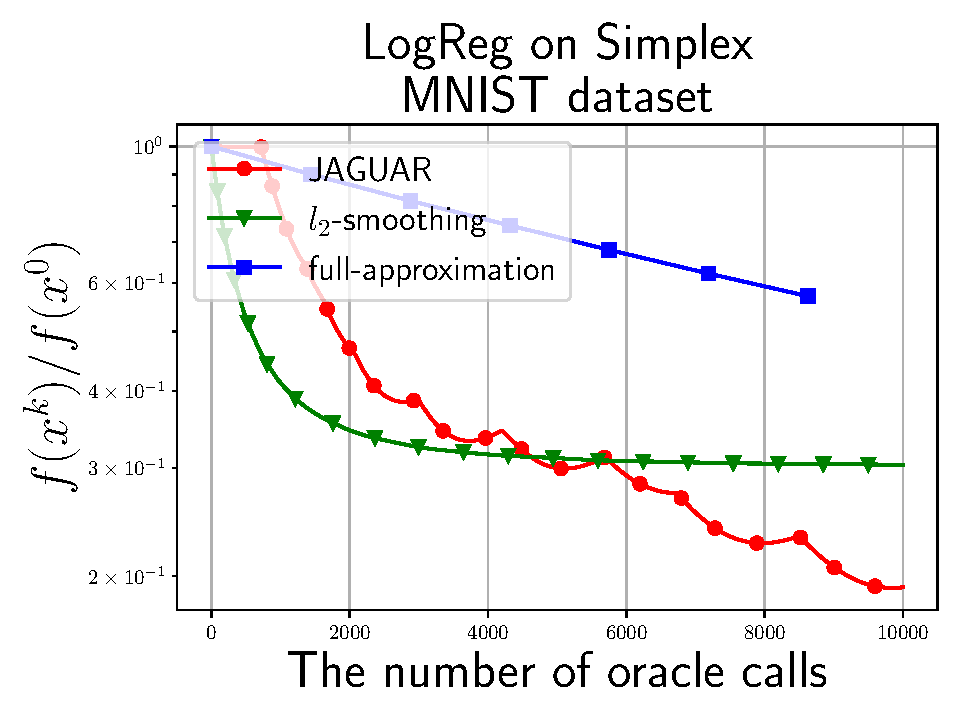
\includegraphics[width=0.49\textwidth]{figures/Stochastics_TPF_FW_LogReg_Simplex_MNIST.pdf}
        
    \end{figure}

\end{frame}

%----------------------------------------------------------------------------------------------------------

\begin{frame}{Выносится на защиту}

    \begin{enumerate}
        \item Предложен робастый алгоритм аппроксимация градиента \texttt{JAGUAR}, использующий $\mathcal{O}(1)$ вызовов оракула на каждой итерации.
        \item Доказаны теоретические оценки сходимости использования данного метода для нестохастического и стохастического случаев в алгоритме Франка-Вульфа. Показано теоретическое превосходство над $l_2$-\textit{сглаживанием} и \textit{полной аппроксимаций}. 
        \item Проведены вычислительные эксперименты, в которых сравнивается \texttt{JAGUAR}-аппроксимация с $l_2$-сглаживанием и полной аппроксимаций на различных задачах минимизации. Показано практическое превосходство.
    \end{enumerate}

\end{frame}

%-----------------------------------------------------------------------------------------------------

\begin{frame}{Литература}
    \begin{itemize}
        \item Marguerite Frank and Philip Wolfe. An algorithm for quadratic programming. Naval research logistics quarterly, 3(1-2):95–110, 1956.
        \item Darina Dvinskikh, Vladislav Tominin, Iaroslav Tominin, and Alexander Gasnikov. Noisy zeroth-order optimization for non-smooth saddle point problems. In International Conference on Mathematical Optimization Theory and Operations Research, pages 18–33. Springer, 2022.
        \item Anit Kumar Sahu, Manzil Zaheer, and Soummya Kar. Towards gradient free and projection free stochastic optimization. In The 22nd International Conference on Artificial Intelligence and Statistics, pages 3468–3477. PMLR, 2019.
    \end{itemize}

\end{frame}

%----------------------------------------------------------------------------------------------------------

\end{document}